
%--- Outline ---
\begin{frame}{Outline}
  \begin{itemize}
    \item What is Image Classification?
    \item How Can We Improve It? (Data Augmentation)
    \item Real-World Example: Disaster Images
    \item Project: Can AI-Generated Images Help?
  \end{itemize}
\end{frame}

% \begin{refsection}
%   \begin{frame}
%     \centering
%     \vspace{2.5cm}
%     {\LARGE \textbf{Introduction to Image Classification}\\[0.5em]
%     \textbf{using Deep Learning}}
%   \end{frame}
% \end{refsection}


\begin{frame}{What is Image Classification?}
  \begin{itemize}
    \item Computers learn to recognize what’s in a picture (e.g., cat, dog, airplane).
    \item We use lots of labeled images to teach the computer.
    \item Goal: Predict the correct label for new images.
  \end{itemize}
  \centering
  \includegraphics[height=0.6\textheight]{image_classification_idea.png}
\end{frame}

%--- End-to-End Neural Network ---
\begin{refsection}
\begin{frame}{End-to-End Neural Network}
  \begin{figure}
    \centering
    \includegraphics[width=1.0\linewidth]{end2end.png}
    \caption[]{\scriptsize An end-to-end neural network for image classification. The image passes through multiple layers, and the network learns by backpropagation. Image Source:~\cite{he2025endtoend}.}
  \end{figure}
  \bottomleftrefs
\end{frame}
\end{refsection}

%--- How Does It Work? ---
\begin{refsection}
\begin{frame}{How Does It Work?}
  \begin{flushleft}
  Neural networks are special computer programs that learn patterns from many example images. Over time, they get better at telling images apart.
  \end{flushleft}
  \centering
  \begin{figure}
    \centering
    \includegraphics[width=0.6\linewidth]{alexnet.png}
    \caption[]{\scriptsize Example of a neural network for image classification: AlexNet~\parencite{krizhevskyImageNetClassificationDeep2012}.}
  \end{figure}
  \bottomleftrefs
\end{frame}
\end{refsection}




%--- Modern Models: CLIP ---
\begin{refsection}
\begin{frame}{Modern Models: CLIP}
  % \vspace{-0.7em}
  \begin{itemize}
    \item CLIP learns to match images and text.
    \item It can recognize new things by understanding descriptions.
    \item Useful for many tasks, not just classification.
  \end{itemize}
  \centering
  \begin{figure}
    \centering
    \includegraphics[width=0.8\linewidth]{clip.png}
    \caption[]{\scriptsize Summary of OpenAI CLIP ViT~\parencite{radfordLearningTransferableVisual2021}.}
  \end{figure}
  \bottomleftrefs
\end{frame}
\end{refsection}



%--- Section: Data Augmentation ---
\begin{refsection}
\begin{frame}
  \centering
  \vspace{2.5cm}
  {\LARGE \textbf{How Can We Improve Image Classification?}\\[0.5em]
  \textbf{(Data Augmentation)}}
\end{frame}
\end{refsection}

%--- Data Augmentation: Why? ---
\begin{refsection}
\begin{frame}{Why Use Data Augmentation?}
  \begin{minipage}{0.48\linewidth}
    \begin{itemize}
      \item Sometimes we do not have enough images to train a good model.
      \item Data augmentation means making new images from existing ones.
      \item It helps the model learn better and avoid mistakes.
    \end{itemize}
  \end{minipage}%
  \hfill
  \begin{minipage}{0.48\linewidth}
    \centering
    \includegraphics[width=0.95\linewidth]{augreg.png}
    \scriptsize \\
    Figure. Adding the right amount of regularization and image augmentation can lead to similar gains as increasing the dataset size by an order of magnitude.~\parencite{steinerHowTrainYour2022}
  \end{minipage}
  \bottomleftrefs
\end{frame}
\end{refsection}

%--- Data Augmentation: How? ---
\begin{refsection}
\begin{frame}{How Do We Augment Data?}
  \textbf{Classic Methods:}
    \begin{itemize}
      \item Flip, rotate, crop, change colors, etc.
    \end{itemize}
    \textbf{Modern Methods:}
    \begin{itemize}
      \item Mix two images together (Mixup)~\parencite{zhangMixupEMPIRICALRISK2018}.
      \item Cut and paste parts of images (CutMix)~\parencite{yunCutMixRegularizationStrategy2019}.
    \end{itemize}
  \begin{minipage}{0.58\linewidth}
    \begin{figure}
      \centering
      \includegraphics[width=0.6\linewidth]{aug_new_methods.png}
      \caption[]{\scriptsize Illustration of modern augmentation methods. From Left to Right: Mixup~\parencite{zhangMixupEMPIRICALRISK2018}, Cutout~\parencite{devriesImprovedRegularizationConvolutional2017}, and CutMix~\parencite{yunCutMixRegularizationStrategy2019}.}
    \end{figure}
  \end{minipage}
  \hfill
  \begin{minipage}{0.4\linewidth}
    \textbf{Soft Label Example (CutMix):}
    % \vspace{0.5em}
    \tiny
    \begin{equation*}
      \text{cutmix\_label} = \lambda \cdot \text{label}_A + (1 - \lambda) \cdot \text{label}_B
    \end{equation*}
    \vspace{-0.5em}
    \begin{equation*}
      \text{Example:} \quad \lambda = 0.5, \quad \text{label}_A = [1, 0], \quad \text{label}_B = [0, 1]
    \end{equation*}
    \vspace{-0.5em}
    \begin{equation*}
      \text{cutmix\_label} = 0.5 \times [1, 0] + 0.5 \times [0, 1] = [0.5, 0.5]
    \end{equation*}
   

  \end{minipage}
  \bottomleftrefs
\end{frame}
\end{refsection}


%--- Example Dataset: RESISC45 ---
% \begin{refsection}
%   \begin{frame}{Example Dataset: RESISC45}
%     \centering
%     \begin{figure}
%       \centering
%       \includegraphics[width=1.0\linewidth]{RESISC45_part2.png}
%       \caption[]{\scriptsize Example images from the RESISC45 dataset~\parencite{Cheng2017}, which contains 45 scene classes with 700 images each.}
%     \end{figure}
%     \bottomleftrefs
%   \end{frame}
%   \end{refsection}

%--- Generative Models for Data Augmentation ---
\begin{refsection}
\begin{frame}{Using Gen AI to Make New Images}
  \begin{itemize}
    \item Generative models can create new, realistic images.
    \item We can use them to make more training data.
    \item Example: Give a “before” image and a description, get a new “after” image.
  \end{itemize}
  \centering
  \includegraphics[width=1.0\linewidth]{diffusion_editing.png}
\end{frame}
\end{refsection}

%--- Real-World Example: Disaster Images (xBD) ---
\begin{frame}
  \centering
  \vspace{2.5cm}
  {\LARGE \textbf{Real-World Example: Disaster Images (xBD)}}
\end{frame}

\begin{refsection}
  \begin{frame}{xBD: A Large-Scale Disaster Damage Dataset}
    \begin{minipage}{0.42\linewidth}
      \centering
      \includegraphics[width=1.0\linewidth]{xbd_samples.png}
      \vspace{0.5em}
      \scriptsize
      \textbf{xBD}~\parencite{guptaCreatingXBDDataset2019} is a bi-temporal remote sensing dataset covering 19 distinct disaster events. Pre-disaster imagery (top) and post-disaster imagery (bottom). From left to right: Hurricane Harvey; Joplin tornado; Lower Puna volcanic eruption; Sunda Strait tsunami.
    \end{minipage}%
    \hfill
    \begin{minipage}{0.55\linewidth}
      \tiny
      \centering
      \textbf{Table. 19 Disaster events in xBD.}
      \begin{tabular}{lll}
        \hline
        \textbf{Disaster Type} & \textbf{Disaster Event} & \textbf{Event Date} \\
        \hline
        Earthquake & Mexico City earthquake & Sep 19, 2017 \\
        Wildfire & Portugal wildfires & Jun 17--24, 2017 \\
        Wildfire & Santa Rosa wildfires & Oct 8--31, 2017 \\
        Wildfire & Carr wildfire & Jul 23--Aug 30, 2018 \\
        Wildfire & Woolsey fire & Nov 9--28, 2018 \\
        Wildfire & Piner fire & Nov 25--Dec 2, 2018 \\
        Volcano & Lower Puna volcanic eruption & May 23--Aug 14, 2018 \\
        Volcano & Guatemala Fuego volcanic eruption & Jun 3, 2018 \\
        Storm & Tuscaloosa, AL tornado & Apr 27, 2011 \\
        Storm & Joplin, MO tornado & May 22, 2011 \\
        Storm & Moore, OK tornado & May 20, 2013 \\
        Storm & Hurricane Matthew & Sep 28--Oct 10, 2016 \\
        Storm & Hurricane Florence & Sep 10--19, 2018 \\
        Flooding & Monsoon in Nepal, India, and Bangladesh & Aug 2017 \\
        Flooding & Hurricane Harvey & Aug 17--Sep 7, 2017 \\
        Flooding & Hurricane Michael & Oct 7--16, 2018 \\
        Flooding & Midwest US floods & Jan 3--May 31, 2019 \\
        Tsunami & Indonesia tsunami & Sep 18, 2018 \\
        Tsunami & Sunda Strait tsunami & Dec 22, 2018 \\
        \hline
      \end{tabular}
      \vspace{0.5em}

    \end{minipage}
    \bottomleftrefs
  \end{frame}
\end{refsection}

%--- Project Section ---
\begin{frame}
  \centering
  \vspace{2.5cm}
  {\LARGE \textbf{Project: Can AI-Generated Images Help?}}
\end{frame}

%--- Project: What Will You Do? ---
\begin{refsection}
\begin{frame}{Project: What Will You Do?}
  \begin{itemize}
    \item Test if adding AI-generated images helps the model learn.
    \item Try three ways:
      \begin{itemize}
        \item Only real images
        \item Only generated images
        \item Both real and generated images
      \end{itemize}
    \item See which way gives the best results!
  \end{itemize}
\end{frame}
\end{refsection}

%--- Project: Dataset & Image Generation ---
\begin{refsection}
\begin{frame}{Project: Dataset Details \& How to Generate Images}
  \begin{itemize}
    \item Use 100 real images per disaster type (6 types, 600 images total).
    \item For each type, generate 100–400 new images using AI.
    \item Try different mixes: 1:1, 1:2, 1:3, 1:4 (real:generated).
    \item Use commercial AI models (e.g., GPT-Image-1~\parencite{gptimage1}, Gemini 2.5 Pro~\parencite{geminiteamgoogleGemini25Pushing}, SeedEdit 3.0~\parencite{wang2025seedit}) to generate images.
    \item Input: a “before” image and a short description (e.g., “make it suffer from flooding”).
    \item Output: a new, realistic “after” image.
  \end{itemize}
  \bottomleftrefs
\end{frame}
\end{refsection}

%--- Project: Models & Evaluation ---
\begin{refsection}
\begin{frame}{Which Models to Use \& How to Measure Success}
  \begin{itemize}
    \item \textbf{Try these models:}
      \begin{itemize}
        \item OpenAI CLIP~\parencite{radfordLearningTransferableVisual2021}
        \item Google SigLip/SigLip2~\parencite{tschannenSigLIP2Multilingual2025,Zhai_2023_ICCV}
        \item Both of the above use ViT configurations (see \href{https://github.com/huggingface/transformers/blob/main/examples/pytorch/contrastive-image-text/README.md}{\textcolor{blue}{CLIP training example}} and \href{https://github.com/NielsRogge/Transformers-Tutorials/tree/master/VisionTransformer}{\textcolor{blue}{ViT tutorials}}).
      \end{itemize}
    \item \textbf{How to measure success:}
      \begin{itemize}
        \item \textbf{Accuracy}: \% of correct answers
        \item \textbf{F1 Score}: balances precision and recall
        \item \textbf{Confusion Matrix}: shows what gets confused
      \end{itemize}
    \item Always test on real images the model hasn’t seen before.
    \item Make simple bar or line charts to compare results.
  \end{itemize}
  \bottomleftrefs
\end{frame}
\end{refsection}

%--- Summary / Key Takeaways ---
% \begin{frame}{Key Takeaways}
%   \begin{itemize}
%     \item Image classification helps computers understand pictures.
%     \item Data augmentation (including AI-generated images) can help models learn better.
%     \item Your project: test if mixing real and generated images improves results!
%     \item Simple experiments and clear results are best.
%   \end{itemize}
% \end{frame}
  

% \begin{refsection}
%   \begin{frame}{Baseline Models for Scene Classification}
%     \textbf{Scene Image Classification:}
%     \begin{itemize}
%       \item \textbf{OpenAI CLIP}~\parencite{radfordLearningTransferableVisual2021}~\href{https://hf-mirror.com/openai/clip-vit-base-patch16}{\textcolor{blue}{- models}}
%       \item \textbf{RemoteCLIP}~\parencite{liuRemoteCLIPVisionLanguage2024}~\href{https://hf-mirror.com/MVRL/remote-clip-vit-base-patch32}{\textcolor{blue}{- models}}
%       \item \textbf{Git-RSCLIP}~\parencite{text2earth2025}~\href{https://hf-mirror.com/lcybuaa/Git-RSCLIP-base}{\textcolor{blue}{- models}}
%     \end{itemize}
%     All of above follow ViT configuration where we can use following~\href{https://github.com/huggingface/transformers/blob/main/examples/pytorch/contrastive-image-text/README.md}{\textcolor{blue}{(code)}}~for continuing CLIP training or ~\href{https://github.com/NielsRogge/Transformers-Tutorials/tree/master/VisionTransformer}{\textcolor{blue}{(code)}}~ for fine-tuning on classification task.
%     For more Remote Sensing Foundation Models, ref to ~\href{https://hf-mirror.com/collections/MVRL/remote-sensing-foundation-models-664e8fcd67d8ca8c03f42d00}{\textcolor{purple}{huggingface collection}.}
%     \bottomleftrefs
%   \end{frame}
%   \end{refsection}



\begin{refsection}
  \begin{frame}[plain]
    \vfill
    \centering
    {\Huge \textbf{Appendix}}
    \vfill
  \end{frame}
\end{refsection}

\begin{refsection}
  \begin{frame}{Background: Image Classification with Deep Learning}
    \begin{figure}
      \centering
      \begin{minipage}{0.48\linewidth}
        \centering
        \includegraphics[width=\linewidth]{imagenet2.png}
      \end{minipage}\hfill
      \begin{minipage}{0.48\linewidth}
        \centering
        \includegraphics[width=\linewidth]{alexnet.png}
      \end{minipage}
      \caption[]{\scriptsize Left: AlexNet on ILSVRC-2010~\parencite{imagenet2010challenge} \quad Right: Architecture of AlexNet~\parencite{krizhevskyImageNetClassificationDeep2012}.}
    \end{figure}
    \bottomleftrefs
  \end{frame}
\end{refsection}



\begin{refsection}
  \begin{frame}{Architecture Evolution of Image Classification}
    \begin{minipage}{0.48\linewidth}
      {\tiny
      \begin{itemize}
        % \item \textbf{2012: AlexNet} \\
        % \parencite{krizhevskyImageNetClassificationDeep2012}
        % \item \textbf{2016: ResNet} \\
        % \parencite{heDeepResidualLearning2016}
        \item \textbf{NeurIPS 2012: AlexNet (CNN)} \\
        \parencite{krizhevskyImageNetClassificationDeep2012}
        \item \textbf{CVPR 2016: ResNet (CNN)} \\
        \parencite{heDeepResidualLearning2016}
        \item \textbf{ICLR 2021: Vision Transformers (ViT)} \\
        \parencite{dosovitskiyImageWorth16x162020}
        \item \textbf{ICCV 2021: Swin Transformer (ViT)} \\
        \parencite{liuSwinTransformerHierarchical2021}
        \item \textbf{ICML 2021: CLIP (ViT)} \\
        \parencite{radfordLearningTransferableVisual2021}
        \item \textbf{CVPR 2022: MAE (ViT)} \\
        \parencite{heMaskedAutoencodersAre2022}
        \item \textbf{TMLR 2022: CoCa (ViT)} \\
        \parencite{yuCoCaContrastiveCaptioners2022}
      \end{itemize}
      }
    \end{minipage}%
    \hfill
    \begin{minipage}{0.48\linewidth}
      \centering
      \includegraphics[width=0.95\linewidth]{vit.png}
      \scriptsize Overview of Vision Transformer\\\parencite{dosovitskiyImageWorth16x162020}.
    \end{minipage}
    \bottomleftrefs
  \end{frame}
\end{refsection}

\begin{refsection}
  \begin{frame}{Image Classification Dataset: RESISC45}
    \begin{figure}
      \centering
      \includegraphics[width=0.95\linewidth]{RESISC45_part2.png}
    \end{figure}
    \scriptsize
    We display 2 example images for each class from the NWPU-RESISC45~\parencite{Cheng2017}, a remote sensing scene classification dataset which consists of 31500 remote sensing images divided into 45 scene classes. Each class includes 700 images with a size of 256 × 256 pixels in RGB.
    \bottomleftrefs
  \end{frame}
\end{refsection}

\begin{refsection}
  \begin{frame}{CLIP for Image Classification}
    \begin{figure}
      \centering
      \includegraphics[width=1.0\linewidth]{clip.png}
      \caption{\scriptsize Summary of OpenAI CLIP ViT~\parencite{radfordLearningTransferableVisual2021}. Left: Training. Right: Inference. }
    \end{figure}
    \bottomleftrefs
  \end{frame}
\end{refsection}

\begin{refsection}
  \begin{frame}
    \centering
    \vspace{2.5cm}
    {\LARGE \textbf{Data Augmentation Methods}}
  \end{frame}
\end{refsection}

\begin{refsection}
  \begin{frame}{Traditional vs. Modern Data Augmentation Methods}
    \textbf{Classic Methods:}
    \begin{itemize}
      \item \textbf{Geometric Transformations:} Rotation, Flipping, Scaling, Translation, Cropping
    \end{itemize}
    \textbf{Modern Methods:}

    \centering
    \includegraphics[width=0.7\linewidth]{aug_new_methods.png}

    \scriptsize
    Illustration of modern augmentation methods. From Left to Right: Mixup~\parencite{zhangMixupEMPIRICALRISK2018}, Cutout~\parencite{devriesImprovedRegularizationConvolutional2017}, and CutMix~\parencite{yunCutMixRegularizationStrategy2019}.

    \bottomleftrefs
  \end{frame}
\end{refsection}

\begin{refsection}
  \begin{frame}{Using Generative Model for Synthetic Dataset for Data Augmentation}
    \begin{minipage}{0.65\linewidth}
      \centering
      \includegraphics[width=0.95\linewidth]{text2earth.png}
      % \vspace{0.5em}
      
    \end{minipage}
    \hfill
    \begin{minipage}{0.33\linewidth}
      \centering
      \includegraphics[width=1.0\linewidth]{text2earth_results2.png}
      % \vspace{0.5em}
      
    \end{minipage}
    \vspace{1em}
    
    \scriptsize
    \textbf{Left:} Text2Earth~\parencite{text2earth2025}, a foundation model for text-driven remote sensing image generation observation. \textbf{Right:} Example results generated by Text2Earth. 
    Generative models such as Text2Earth can be used to create synthetic remote sensing images, which can augment real datasets for tasks like image scene classification.
    \bottomleftrefs
  \end{frame}
\end{refsection}

\begin{refsection}
  \begin{frame}
    \centering
    \vspace{2.5cm}
    {\LARGE \textbf{Remote Sensing Temporal Dataset}\\[0.5em]
    \textbf{for Disaster Events: xBD}}
  \end{frame}
\end{refsection}



\begin{refsection}
  \begin{frame}
    \centering
    \vspace{2.5cm}
    {\LARGE \textbf{Project: Explore whether generated images can benefit image classification}}
  \end{frame}
\end{refsection}

\begin{refsection}
  \begin{frame}{Project Assignment: Overview}
    \textbf{Project: Can Generated Images Improve Remote Sensing Image Classification?}
  
    \vspace{0.7em}
    \textbf{Objective:}\\
    Investigate whether combining real images and generated images can improve remote sensing image classification.

    \vspace{1em}
    \textbf{Pipeline:}\\
    In this project, you will experiment with three different training settings to evaluate the impact of generated data:
    \begin{enumerate}
      \item \textbf{Real Dataset Only:} Train the classification model using only real images from the xBD dataset.
      \item \textbf{Generated Dataset Only:} Train the model using only synthetic images generated by commercial generative models.
      \item \textbf{Combined Dataset:} Train the model using both real and generated images together.
    \end{enumerate}
    Compare the classification performance across these three settings to analyze the effect of synthetic data.

    \bottomleftrefs
  \end{frame}
\end{refsection}
  
%--- Slide: Dataset ---
\begin{refsection}
  \begin{frame}{Project Assignment: Dataset}
    \textbf{Dataset: xBD Disaster Damage Dataset}
    \begin{itemize}
      \item Use the \textbf{xBD} remote sensing disaster dataset.
      \item The dataset includes \textbf{6 disaster classes}.
      \item For each class, use \textbf{100 real images} (total: 600 real images).
    \end{itemize}
    \bottomleftrefs
  \end{frame}
  \end{refsection}
  
  %--- Slide: Generative Models ---
  \begin{refsection}
    \begin{frame}{Project Assignment: Generative Models}
      \textbf{Image Generation:}
      \begin{itemize}
        \item We consider generated images as the result of \textbf{text-guided image editing}: for each case, you input a \textbf{pre-event image} and a \textbf{text description} (e.g., "flooded", "collapsed building"), and the model yields a generated (post-event) image.
        \item Use commercial generative models such as \textbf{GPT-4o Image Generation(GPT-Image-1)}~\parencite{gptimage1}, \textbf{Gemini-2}~\parencite{geminiteamgoogleGemini25Pushing}, or \textbf{SeedEdit 3.0}~\parencite{wang2025seedit} to create synthetic images for each disaster class.
      \end{itemize}
      \bottomleftrefs
    \end{frame}
  \end{refsection}
  
  
  %--- Slide: Classification Models ---
  \begin{refsection}
  \begin{frame}{Project Assignment: Classification Models}
    \textbf{Recommended Baseline Models:}
    \begin{itemize}
      \item \textbf{OpenAI CLIP}~\parencite{radfordLearningTransferableVisual2021}~\href{https://hf-mirror.com/openai/clip-vit-base-patch16}{\textcolor{blue}{- models}}
      \item \textbf{RemoteCLIP}~\parencite{liuRemoteCLIPVisionLanguage2024}~\href{https://hf-mirror.com/MVRL/remote-clip-vit-base-patch32}{\textcolor{blue}{- models}}
      \item \textbf{Git-RSCLIP}~\parencite{text2earth2025}~\href{https://hf-mirror.com/lcybuaa/Git-RSCLIP-base}{\textcolor{blue}{- models}}
    \end{itemize}
    \vspace{0.5em}
    All of the above follow ViT configurations. For code and tutorials:
    \begin{itemize}
      \item \href{https://github.com/huggingface/transformers/blob/main/examples/pytorch/contrastive-image-text/README.md}{\textcolor{blue}{CLIP training example}}
      \item \href{https://github.com/NielsRogge/Transformers-Tutorials/tree/master/VisionTransformer}{\textcolor{blue}{ViT tutorials}}
      \item For more Remote Sensing Foundation Models, ref to ~\href{https://hf-mirror.com/collections/MVRL/remote-sensing-foundation-models-664e8fcd67d8ca8c03f42d00}{\textcolor{purple}{huggingface collection}.}
      \item The latest strong baseline RSFM 'SkySense-O'~\parencite{zhuSkySenseOOpenWorldRemote2025}. \href{https://github.com/zqcrafts/SkySense-O}{\textcolor{blue}{GitHub}}

    \end{itemize}
    \bottomleftrefs
  \end{frame}
  \end{refsection}
  
  %--- Slide: Data Augmentation Protocol ---
  \begin{refsection}
  \begin{frame}{Project Assignment: Data Augmentation Protocol}
    \begin{itemize}
      \item For each disaster class, generate \textbf{1$\times$--4$\times$} synthetic images (i.e., 100, 200, 300, or 400 synthetic images per class).
      \item Explore and compare different ratios of real to synthetic images (e.g., 1:1, 1:2, 1:3, 1:4).
      \item The augmented dataset for each class will range from \textbf{200 to 500 images}.
    \end{itemize}
    \bottomleftrefs
  \end{frame}
  \end{refsection}
  
  %--- Slide: Evaluation ---
  \begin{refsection}
  \begin{frame}{Project Assignment: Evaluation}
    \textbf{Evaluation:}
    \begin{itemize}
      \item Use \textbf{standard accuracy}, \textbf{F1 score}, and \textbf{confusion matrix} to measure performance.
      \item Always evaluate on a \textbf{held-out real (unseen) test set}.
      \item Include \textbf{curve or bar plots} comparing classification performance across different real:synthetic ratios.
    \end{itemize}
    \bottomleftrefs
  \end{frame}
  \end{refsection}

\begin{refsection}
  \begin{frame}{Traditional Data Augmentation Methods}
    \begin{itemize}
      \item \textbf{Geometric Transformations:} \textbf{Rotation}, \textbf{Flipping} (horizontal/vertical), \textbf{Scaling}, \textbf{Translation}, \textbf{Cropping}
      \item \textbf{Color Jittering:} Adjusting brightness, contrast, saturation, and hue
      \item \textbf{Noise Injection:} Adding random noise to images
      \item \textbf{Cutout}~\parencite{devriesImprovedRegularizationConvolutional2017}
      \item \textbf{CutMix}~\parencite{yunCutMixRegularizationStrategy2019}
      \item \textbf{Copy-Paste}~\parencite{ghiasiSimpleCopyPasteStrong2021}
    \end{itemize}
    There is also a comprehensive study entitled 'How to train your ViT? Data, Augmentation,  and Regularization in Vision Transformers'~\parencite{steinerHowTrainYour2022}.
    \bottomleftrefs
  \end{frame}
\end{refsection}

\begin{refsection}
  \begin{frame}{Generative Models for Data Augmentation}
    \begin{minipage}{0.7\linewidth}
      % \centering
      \includegraphics[width=0.9\linewidth]{satsyn.png}
    \end{minipage}%
    \hfill
    \begin{minipage}{0.3\linewidth}
      \scriptsize
      SatSyn~\parencite{tokerSatSynthAugmentingImageMask2024} proposes a generative model (diffusion model) to generate both images and corresponding masks for satellite segmentation. The synthetic dataset is used for data augmentation, yielding significant quantitative improvements in satellite semantic segmentation compared to other data augmentation methods.
    \end{minipage}
    \bottomleftrefs
  \end{frame}
\end{refsection}

\begin{refsection}
  \begin{frame}{Generated Text-Image Dataset Improving Image Classification}
    \centering
    \includegraphics[width=0.8\linewidth]{syn_aug_results.png}
    
    % \vspace{0.5em}
    
    \scriptsize
    Synthetic text-image datasets generated by generative models can significantly improve image classification performance, as demonstrated in~\parencite{heSYNTHETICDATAGENERATIVE2022}.
    \bottomleftrefs
  \end{frame}
\end{refsection}

  %--- Slide: Datasets for Text-to-Image Generation ---
  \begin{refsection}
    \begin{frame}{Additonal Text-Image Remote Sensing Datasets}
      \textbf{Text-to-Image Generation:}
      \begin{itemize}
        \item \textbf{RSICD}~\parencite{lu2017exploring}: Remote Sensing Image Captioning Dataset with 10,921 images and five captions per image.
        \item \textbf{RSICap}~\parencite{hu2023rsgpt}: High-quality dataset with 2,585 human-annotated image-caption pairs.
        \item \textbf{UCM-Captions}~\parencite{qu2016deep}: Derived from the UC Merced Land Use Dataset, containing 2,100 images with five captions each.
        \item \textbf{RESISC45}~\parencite{Cheng2017}: It is a publicly available benchmark for REmote Sensing Image Scene Classification (RESISC), created by Northwestern Polytechnical University (NWPU). This data set contains 31 500 images, covering 45 scene classes with 700 images in each class.
      \end{itemize}
      \bottomleftrefs
    \end{frame}
  \end{refsection}

\begin{refsection}
  \begin{frame}{Generative Modeling}
    \begin{figure}
      \centering
      \includegraphics[width=0.8\linewidth]{learning_to_generate_data.png}
      \caption{\scriptsize Illustration of generative modeling~\parencite{CVPR2023Tutorial}.}
    \end{figure}
    \bottomleftrefs
  \end{frame}
  \end{refsection}
  
  % --- Slide 2: Timeline of Generative Models ---
  \begin{refsection}
  \begin{frame}{Timeline of Generative Models}
    \begin{figure}
      \centering
      \includegraphics[width=0.95\linewidth]{genai_timeline.png}
      \caption{\scriptsize Timeline of key developments in generative models~\parencite{dengPPTAdvancedNueralNetwork2024}.}
    \end{figure}
    \bottomleftrefs
  \end{frame}
  \end{refsection}
  
  
  
  \begin{refsection}
  \begin{frame}{Background: Diffusion Models}
  
    \begin{figure}
      \begin{minipage}{0.95\linewidth}
        \footnotesize
        \textbf{Denoising diffusion models consist of two processes:}
        \begin{itemize}
          \item A forward diffusion process that gradually adds noise to the input.
          \item A reverse denoising process that learns to generate data by denoising.
        \end{itemize}
      \end{minipage}
      \vspace{2em}
  
      \centering
      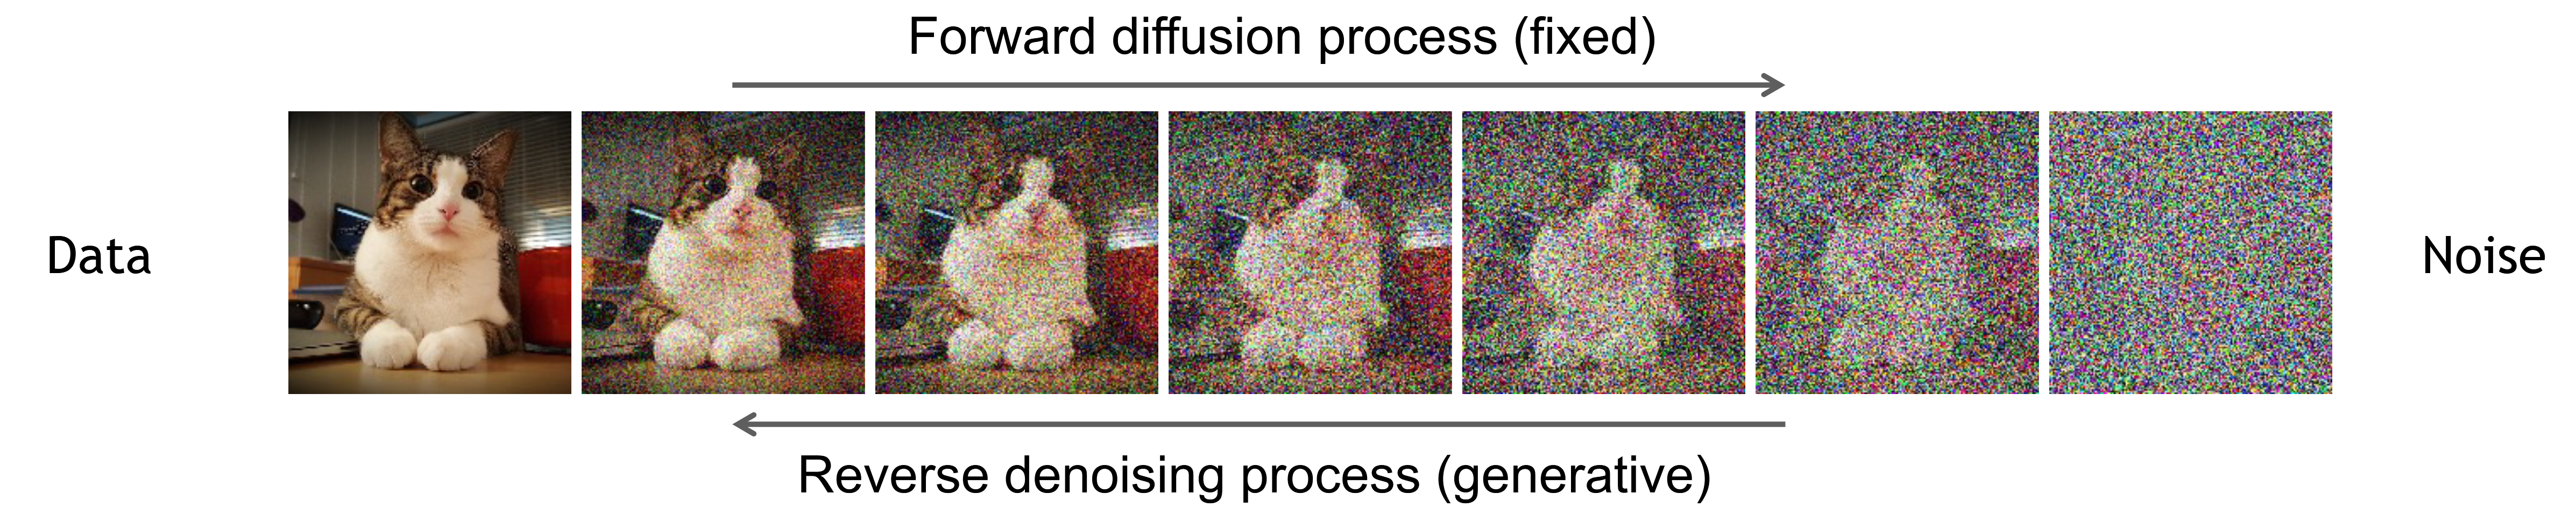
\includegraphics[width=1.0\linewidth]{diffusion_high_level.png}
  
      \caption[]{\scriptsize Diffusion models generate data through iterative denoising~\parencite{sohl2015deep,ho2020denoising}.}
    \end{figure}
  
    \bottomleftrefs
  \end{frame}
  \end{refsection}
  
  % --- Slide 4: Preliminaries of Diffusion Models ---
  \begin{refsection}
  \begin{frame}{Diffusion Models: Forward and Reverse Processes}
    \footnotesize
    \textbf{Forward (Diffusion) Process:}
    \begin{align*}
      q(\mathbf{x}_t \mid \mathbf{x}_{t-1}) &= \mathcal{N}(\mathbf{x}_t; \sqrt{1-\beta_t}\,\mathbf{x}_{t-1}, \beta_t \mathbf{I}) \\
      q(\mathbf{x}_{1:T} \mid \mathbf{x}_0) &= \prod_{t=1}^T q(\mathbf{x}_t \mid \mathbf{x}_{t-1}) \\
      &\text{Equivalently,  } 
      \mathbf{x}_t = \sqrt{\bar{\alpha}_t}\,\mathbf{x}_0 + \sqrt{1-\bar{\alpha}_t}\,\boldsymbol{\epsilon}, \quad \boldsymbol{\epsilon} \sim \mathcal{N}(\mathbf{0}, \mathbf{I})
    \end{align*}
  
    \footnotesize
    \textbf{Reverse (Denoising) Process:}
    \begin{align*}
      p_\theta(\mathbf{x}_{t-1} \mid \mathbf{x}_t) &= \mathcal{N}(\mathbf{x}_{t-1}; \boldsymbol{\mu}_\theta(\mathbf{x}_t, t), \Sigma_\theta(\mathbf{x}_t, t)) \\
      p_\theta(\mathbf{x}_{0:T}) &= p(\mathbf{x}_T) \prod_{t=1}^T p_\theta(\mathbf{x}_{t-1} \mid \mathbf{x}_t)
    \end{align*}
    \scriptsize
    where $\mathbf{x}_0$ is the data, $\beta_t$ is the noise schedule, and $\bar{\alpha}_t = \prod_{s=1}^t (1-\beta_s)$. $p(\mathbf{x}_T) = \mathcal{N}(\mathbf{0}, \mathbf{I})$.
  
    \scriptsize
    \textbf{Diffusion models generate data by learning to reverse a gradual noising process.}~\parencite{sohl2015deep,ho2020denoising}
    \bottomleftrefs
  \end{frame}
  \end{refsection}
  
  \begin{refsection}
  \begin{frame}{Diffusion Models: Training and Inference}
    \footnotesize
    \textbf{Training Objective:}
    \begin{align*}
      \mathcal{L}_{\mathrm{simple}} = \mathbb{E}_{\mathbf{x}_0, \boldsymbol{\epsilon}, t} \left[ \left\| \boldsymbol{\epsilon} - \boldsymbol{\epsilon}_\theta(\sqrt{\bar{\alpha}_t}\mathbf{x}_0 + \sqrt{1-\bar{\alpha}_t}\boldsymbol{\epsilon}, t) \right\|^2 \right]
    \end{align*}
    where $\boldsymbol{\epsilon} \sim \mathcal{N}(\mathbf{0}, \mathbf{I})$, $\bar{\alpha}_t = \prod_{s=1}^t (1-\beta_s)$.
  
    \vspace{0.5em}
    \textbf{Inference (Sampling):}
    \begin{itemize}
      \item Start from pure noise: $\mathbf{x}_T \sim \mathcal{N}(\mathbf{0}, \mathbf{I})$
      \item For $t = T, \ldots, 1$:
        \begin{itemize}
          \item Predict noise: $\boldsymbol{\epsilon}_\theta(\mathbf{x}_t, t)$
          \item Compute mean: $\boldsymbol{\mu}_\theta(\mathbf{x}_t, t)$
          \item Sample: $\mathbf{x}_{t-1} \sim \mathcal{N}(\boldsymbol{\mu}_\theta(\mathbf{x}_t, t), \Sigma_\theta(\mathbf{x}_t, t))$
        \end{itemize}
      \item Repeat until $\mathbf{x}_0$ (generated sample)
    \end{itemize}
  
    \vspace{0.5em}
    \scriptsize
    \textbf{Training:} Minimize the simplified objective~\parencite{ho2020denoising}.\\
    \textbf{Inference:} Iteratively denoise from random noise to generate data.
    \bottomleftrefs
  \end{frame}
  \end{refsection}
  
  %--- Slide 5: Application in Remote Sensing Image Generation: DiffusionSat, CRS-Diff, Text2Earth ---
  
  \begin{refsection}
    \begin{frame}{Application in Remote Sensing Image Generation: Text2Earth}
      \begin{figure}
        \centering
        \includegraphics[width=0.9\linewidth]{text2earth.png}
        \caption[]{\scriptsize Text2Earth: Foundation model for text-driven Earth observation~\parencite{text2earth2025}.}
      \end{figure}
      \bottomleftrefs
    \end{frame}
  \end{refsection}
  
  \begin{refsection}
    \begin{frame}{Text2Earth: Example Results}
      \begin{figure}
        \centering
        \includegraphics[width=0.9\linewidth]{text2earth_results.png}
        \caption[]{\scriptsize Example results generated by Text2Earth~\parencite{text2earth2025}.}
      \end{figure}
      \bottomleftrefs
    \end{frame}
  \end{refsection}
  
  \begin{refsection}
  \begin{frame}{Application in Remote Sensing Image Generation: CRS-Diff}
    \begin{figure}
      \centering
      \includegraphics[width=0.9\linewidth]{crsdiff.png}
      \caption[]{\scriptsize CRS-Diff: Controllable remote sensing image generation framework~\parencite{tang2024crsdiff}.}
    \end{figure}
    \bottomleftrefs
  \end{frame}
  \end{refsection}
  
  \begin{refsection}
  \begin{frame}{CRS-Diff: Example Results}
    \begin{figure}
      \centering
      \includegraphics[width=0.9\linewidth]{crsdiff_results.png}
      \caption[]{\scriptsize Example results generated by CRS-Diff~\parencite{tang2024crsdiff}.}
    \end{figure}
    \bottomleftrefs
  \end{frame}
  \end{refsection}
  
  
  %--- Slide 6a: DiffusionSat Framework ---
  \begin{refsection}
  \begin{frame}{DiffusionSat: Framework Overview}
    \begin{figure}
      \centering
      \includegraphics[width=0.9\linewidth]{diffusionsat.png}
      \caption[]{\scriptsize DiffusionSat: A generative foundation model for satellite imagery~\parencite{diffusionset2024}.}
    \end{figure}
    \bottomleftrefs
  \end{frame}
  \end{refsection}
  
  %--- Slide 6b: DiffusionSat for Super-Resolution ---
  \begin{refsection}
  \begin{frame}{DiffusionSat: Super-Resolution Results}
    \begin{figure}
      \centering
      \includegraphics[width=0.9\linewidth]{diffusionsat_sr_results.png}
      \caption[]{\scriptsize Example results: DiffusionSat for multi-spectral super-resolution~\parencite{diffusionset2024}.}
    \end{figure}
    \bottomleftrefs
  \end{frame}
  \end{refsection}
  
  %--- Slide 6c: DiffusionSat for Inpainting ---
  \begin{refsection}
  \begin{frame}{DiffusionSat: Inpainting Results}
    \begin{figure}
      \centering
      \includegraphics[width=0.9\linewidth]{diffusionsat_inpainting_results.png}
      \caption[]{\scriptsize Example results: DiffusionSat for remote sensing image inpainting~\parencite{diffusionset2024}.}
    \end{figure}
    \bottomleftrefs
  \end{frame}
  \end{refsection}

 